\subsection{Coverings of locally connected spaces}

Let B be a topological space and let E be a B-space. Suppose that its projection p is an étale and separated map.

If the space B is locally connected, the space E is locally connected. If the space E is locally connected, the open subset \(p(\mathrm{E})\) of B (cf. I, p. 29, remark 2) is locally connected.

The image \(s(\mathrm{B})\) of any section \(s\) of \(p\) is open (I, p. 30, cor. 3) and closed in B (I, p. 27, prop. 3). If B is connected and nonempty, it is therefore a connected component of E; in general, it is a union of connected components of E.

If B is locally connected, the union of the images of the sections of p is therefore an open and closed subset of E (cf. TG, I, p. 85).

Suppose that E is a trivializable covering of B, and let \(g: E \to B \times F\) be a trivialization. If the space B is connected, the sets \(V_{x} = \overline{g}^{1}(B \times \{x\})\) as x runs through F, are the connected components of E (cf. prop. 1 of I, p. 69).

PROPOSITION 6. --- Let B be a topological space and let E be a B-space; denote its projection by p. Suppose that the space E is locally connected. For E to be a covering of B, it is necessary and sufficient that every point of B have an open neighborhood U such that the map p induces a homeomorphism from every connected component of \(\overline{p}^{1}(U)\) onto U.

Let \(b\) be a point of B. If E is a covering of B, every open neighborhood U of \(b\) which is connected and over which the covering E is trivializable satisfies the conditions stated in the proposition. Conversely, let U be an open neighborhood of \(b\) satisfying these conditions. The set \(\overline{p}^{1}(\mathrm{U})\) is open; its connected components are open subsets of E (TG, I, p. 85, prop. 11) and form a partition of \(\overline{p}^{1}(\mathrm{U})\). The proposition therefore follows from Corollary 1 (I, p. 70) of Proposition 1.

COROLLARY 1. — Let B be a locally connected topological space, let (E,p) be a covering of B, and let E' be an open and closed subset of E. The B-space (E',p \textbar{} E') is a covering, and p(E') is both open and closed in B.

The spaces E and E′ are locally connected. For every open subset U of B, the set \(\mathrm{E}'\cap\overline{p}^{1}(\mathrm{U})\) is open and closed in \(\overline{p}^{1}(\mathrm{U})\), therefore it is a union of connected components of \(\overline{p}^{1}(\mathrm{U})\). The open subsets U of B such that p induces a homeomorphism from each connected component of \(\overline{p}^{1}(\mathrm{U})\) onto U cover B. By the proposition, \(p\mid E'\) makes \(E'\) a covering of B. The second assertion follows from this (cf. I, p. 68).

COROLLARY 2. --- Let B be a locally connected topological space, let (E,p), (E',p') be coverings of B, and let f,g: E' → E be B-morphisms. For every point b of B, denote \(f_b,g_b\) : \(\mathrm{E}_b\to \mathrm{E}_b'\) the maps induced by f and g, respectively. The set of points b in B such that \(f_b = g_b\) is open and closed in B.

Let X be the set of points x in \(E'\) such that \(f(x) = g(x)\). This is the set of points where the lifts f and g of \(p'\) to E coincide; hence X is open and closed in \(E'\) (prop. 11 of I, p. 34). The complement Y of X is also open and closed; consequently \(p(Y)\) is open and closed in B (corollary 1). Its complement, which is the set of points b of B such that \(f_{b} = g_{b}\) , is therefore also open and closed.

COROLLARY 3. --- Let B be a connected and locally connected topological space, and let (E, p) and (E', p') be coverings of B. For every point b of B, the map \(f \mapsto f_b\) from \(\mathcal{C}_{\mathrm{B}}(\mathrm{E}'; \mathrm{E})\) to \(\mathcal{C}(\mathrm{E}_b'; \mathrm{E}_b)\) is injective.

Let \(b\) be a point of B. Let \(f\) and \(g\) be B-morphisms from E' to E such that \(f_b = g_b\). The set of points \(a\) of B such that \(f_a = g_a\) is open and closed in B (corollary 2) and contains b. It is therefore equal to B, and f is equal to g.

COROLLARY 4. --- Let B be a connected and locally connected topological space, let (E, p) be a covering of B, and let b be a point of B. For E to be a trivializable covering, it is necessary and sufficient that every point of the fiber \(E_{b}\) belong to the image of a continuous section of p.

The condition is necessary. Let \(E'\) be the union of the images of the continuous sections of p, and let \(E''\) be its complement in E. The set \(E'\) is open and closed in E (cf. I, p. 79). Consequently, \((\mathrm{E}', p \mid \mathrm{E}')\) is a covering of B (Corollary 1), and this covering is trivializable by virtue of Corollary 2 (I, p. 70). Suppose that \(E'\) contains \(E_b\) and let us prove that \(E''\) is empty. Since \(E''\) is open and closed in E, \(p(\mathrm{E}'')\) is open and closed in B (corollary 1). Since B is connected and b does not belong to \(p(\mathrm{E}'')\), \(p(\mathrm{E}'') = \varnothing\), therefore \(E'' = \varnothing\).

COROLLARY 5. --- Let

\pandocbounded{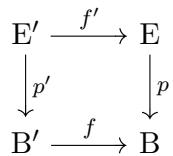
\includegraphics[keepaspectratio]{images/part001_2db9b8ac.jpg}}

a Cartesian square. Suppose that the B-space (E, p) is a covering and that the space B' is connected and locally connected. Let b' be a point of B'. For the B'-space (E', p') to be a trivializable covering, it is necessary and sufficient that for every point x of E such that \(p(x) = f(b')\) there exists a continuous lifting \(g: B' \to E\) of f such that \(g(b') = x\).

Recall that \((\mathrm{E}^{\prime}, p^{\prime})\) is a covering of \(B^{\prime}\) (I, p. 71, cor. 2) and that the map \(f^{\prime}\) induces a bijection \(E_{b^{\prime}}^{\prime} \to E_{f(b^{\prime})}\) (I, p. 10, cor.). By prop. 3 of I, p. 9, the map \(s \mapsto f^{\prime} \circ s\) defines a bijection between the set of continuous sections of \(p^{\prime}\) and the set of continuous lifts of f to E. The corollary therefore follows from Corollary 4.

PROPOSITION 7. --- Let B be a topological space, let E and E' be B-spaces, and let f: E' → E be a B-morphism. Suppose that E' is a covering of B and that the space B is locally connected.

\begin{enumerate}
\def\labelenumi{\alph{enumi})}
\item
  If the projection of the B-space E is an étale and separated map, \((\mathrm{E}^{\prime}, f)\) is a covering of E.
\item
  If f is surjective, then E is a covering of B.
\end{enumerate}

Denote by \(p\) and \(p'\) the projections of the B-spaces E and E′ respectively. Under hypothesis \(a\), \(f\) is étale (I, p. 29, prop. 6, c)). Under hypothesis \(b\), \(p\) is étale (loc. cit., d)). Consequently, under either of these two hypotheses, E is locally connected; its connected components are in particular open and closed in E (TG, I, p. 85, prop. 11).

We shall first prove Proposition 7 under the additional assumption that B is connected, locally connected, and that E' is the trivial covering (B × F', pr₁).

Lemma. --- If U is a connected component of E', the restriction of f to U induces a homeomorphism from U onto a connected component of E.

Let \(x \in F'\) such that \(U = B \times \{x\}\) (cf. I, p. 79). The map from B to E that sends \(b \in B\) to \(f(b, x)\) is a continuous section of p. Its image X is therefore connected and open in E, since p is étale (I, p. 30, cor. 3). It is moreover closed under hypothesis a), since p is separated (I, p. 27, prop. 3). It is also closed under hypothesis b) by Corollary 1 of I, p. 80, since U is open and closed in E'. Consequently, X is a connected component of E.

Since \(f \mid \mathrm{U} \colon \mathrm{U} \to \mathrm{X}\) is bijective and open, it is a homeomorphism onto its image, which proves the lemma.

Let us keep the hypotheses preceding the lemma and now prove assertion \(a\) ). Let V be a connected component of E. It is an open and closed set in E, and \(f^{-1}(\mathrm{V})\) is a union of connected components of \(\mathrm{E}'\) which \(f\) maps homeomorphically onto V by the lemma. It follows from prop. 6 of I, p. 79 that \((\mathrm{E}', f)\) is a covering.

Let us prove b). Since f is surjective, it follows from the lemma that every connected component V of E is the homeomorphic image of a connected component \(U = B \times \{x\}\) of \(E'\) . The map p then induces a homeomorphism from V onto B. By prop. 6, E is a covering of B.

This therefore proves the proposition, under the additional hypothesis that B is connected and E' is a trivializable covering of B. Let us prove it in the general case.

There exists a covering \((\mathrm{U}_{i})_{i\in\mathrm{I}}\) of B, consisting of connected open sets over which the covering \(E'\) is trivializable. Let \(i\in I\) .

Let us prove \(a\). If the map \(p\) is étale and separated, the same is true of the map \(p_{\mathrm{U}_i}\colon \mathrm{U}_i\times_{\mathrm{B}}\mathrm{E}\to \mathrm{U}_i\), for \(i\in \mathrm{I}\), by props. 8 of I, p. 31 and 4 of I, p. 27. It follows therefore from the particular case treated that, for every \(i\in \mathrm{I}\), the \(\mathrm{U}_i\)-space \((\overline{p'}^{1}(\mathrm{U}_i),f_{\mathrm{U}_i})\) is a covering. Let A denote the total space of the disjoint union \(\coprod_{i\in I}\mathrm{U}_i\) and \(q\colon \mathrm{A}\to \mathrm{B}\) the canonical map. Then, the space \(\mathrm{A}\times_{\mathrm{B}}\mathrm{E}'\), equipped with the map \(f_{\mathrm{A}}\colon \mathrm{A}\times_{\mathrm{B}}\mathrm{E}'\to \mathrm{A}\times_{\mathrm{B}}\mathrm{E}\), is a covering of \(\mathrm{A}\times_{\mathrm{B}}\mathrm{E}\). The map \(q\) admits a continuous section in a neighborhood of every point of B, and Proposition 3 of I, p. 72, applied to the Cartesian square

\[
\begin{array}{c} \mathrm {A\times_ {B} E^ {\prime}} \longrightarrow \mathrm {E^ {\prime}} \\ \Big \downarrow f _ {\mathrm{A}} \\ \mathrm {A\times_ {B} E} \longrightarrow \mathrm{E} \end{array} ,
\]

implies that \(E'\) is a covering of E.

Let us prove \(b\). Suppose that \(f\) is surjective. Then, for every element \(i\) from I, the map \(f_{\mathrm{U}_i}\colon \mathrm{U}_i\times_{\mathrm{B}}\mathrm{E}'\to \mathrm{U}_i\times_{\mathrm{B}}\mathrm{E}\) is surjective and the space \(\mathrm{U}_i\times_{\mathrm{B}}\mathrm{E}'\), equipped with the map \(f_{\mathrm{U}_i}\), is a covering of \(\mathrm{U}_i\times_{\mathrm{B}}\mathrm{E}\) (I, p. 71, cor. 2 of prop. 2). From the special case treated previously, it follows that the \(\mathrm{U}_i\)-space \((\overline{p}^{1}(\mathrm{U}_{i}),p_{\mathrm{U}_{i}})\) is a covering. Consequently, E is a covering of B.

Let B be a topological space, let E and E′ be coverings of B, and let \(f: E \rightarrow E'\) be a B-morphism. We have seen that \((E, f)\) is a covering under each of the following two hypotheses: 1) the covering E is locally of finite degree (I, p. 76, cor. 1); 2) the space B is locally connected (I, p. 81, prop. 7). This phenomenon can be explained as follows.

Let F and F′ be discrete topological spaces, and let \(f: B \times F \to B \times F'\) be a B-morphism. The map \(\widetilde{f}: b \mapsto \mathrm{pr}_{2} \circ f(b, \cdot)\) from B to the space \(\mathcal{C}_{c}(F; F')\) is continuous (TG, X, p. 28, th. 3). If U is an open subset of B such that the map \(\widetilde{f}\) is constant on U, the map \(f_{U}: U \times F \to U \times F'\) deduced from f is a trivializable covering (I, p. 69, prop. 1).

The space \(\mathcal{C}_c(\mathrm{F};\mathrm{F}')\) is none other than the set \(\mathcal{F}(\mathrm{F};\mathrm{F}')\) of maps from F into \(\mathrm{F}'\) endowed with the topology induced by the topology of the product space \((\mathrm{F}')^{\mathrm{F}}\) by the canonical identification. For this topology, the space \(\mathcal{F}(\mathrm{F};\mathrm{F}')\) is totally disconnected (I, p. 84, prop. 10). Consequently, if the space B is connected, the map \(\widetilde{f}\) is constant (I, p. 82, prop. 4); if the space B is locally connected, the map \(\widetilde{f}\) is locally constant. When the set F is finite, the space \(\mathcal{F}(\mathrm{F};\mathrm{F}')\) is discrete and the map \(\widetilde{f}\) is locally constant.

Remark. --- Let B be a topological space, let \((\mathrm{E}, p)\) and \((\mathrm{E}', p')\) be B-spaces and let \(f: E' \to E\) be a B-morphism.

\begin{enumerate}
\def\labelenumi{\alph{enumi})}
\item
  If E and E' are coverings of B, the map f is étale (I, p. 29, prop. 6) and separated (I, p. 25, prop. 2). But it is not true in general that (E', f) is a covering of E if the space B is not locally connected (I, p. 145, exerc. 4).
\item
  If \((\mathrm{E}^{\prime}, p^{\prime})\) is a covering of B, f is surjective and makes \(E^{\prime}\) a covering of E, then the map p is étale (I, p. 29, prop. 6). But it is not true, in general, that it is separated if the space B is not locally connected (I, p. 145, exerc. 4). In particular, E is not necessarily a covering of B.
\end{enumerate}

COROLLARY. --- Let B be a connected and locally connected topological space. Let E and E' be coverings of B. Let b be a point of B. Let \(f: E' \to E\) be a B-morphism and let \(f_{b}: E_{b}' \to E_{b}\) be the map induced by f by restriction to the fibers. If the map \(f_{b}\) is injective (resp. surjective, resp. bijective), then so is the map f.

Denote by \(p\) the projection of the B-space E. According to the proposition, \((\mathrm{E}', f)\) is a covering of E; its image \(f(\mathrm{E}')\) is open and closed in E. Let U denote the complement of \(f(\mathrm{E}')\) in E, so that the B-space \((\mathrm{U}, p \mid \mathrm{U})\) is a covering of B (I, p. 80, corollary 1). If the map \(f_b\) is surjective, the fiber at \(b\) of this covering is empty. Since B is a connected space, U is then empty, so \(f\) is surjective.

The set V of points of E where the fiber of f has exactly one element is open and closed. The B-spaces \((V, p|V)\) and \((f(E'), p|f(E'))\) are coverings of B (loc. cit.) and the canonical map \(i: V \to f(E')\) is a B-morphism. If the map \(f_b\) is injective, the map \(i_b\) is surjective, hence i is surjective by the preceding result, and we have \(V = f(E')\). Consequently, the map f is injective.

